%% ****** Start of file apstemplate.tex ****** %
%%
%%   This file is part of the APS files in the REVTeX 4 distribution.
%%   Version 4.1r of REVTeX, August 2010
%%
%%
%%   Copyright (c) 2001, 2009, 2010 The American Physical Society.
%%
%%   See the REVTeX 4 README file for restrictions and more information.
%%
%
% This is a template for producing manuscripts for use with REVTEX 4.0
% Copy this file to another name and then work on that file.
% That way, you always have this original template file to use.
%
% Group addresses by affiliation; use superscriptaddress for long
% author lists, or if there are many overlapping affiliations.
% For Phys. Rev. appearance, change preprint to twocolumn.
% Choose pra, prb, prc, prd, pre, prl, prstab, prstper, or rmp for journal
%  Add 'draft' option to mark overfull boxes with black boxes
%  Add 'showpacs' option to make PACS codes appear
%  Add 'showkeys' option to make keywords appear
\documentclass[10pt,%
               aps,%
               prl,%
               preprint,%
               superscriptaddress,%
               preprintnumbers,%
               amsmath,%
               floatfix,%
               endfloats*]{revtex4-1}
\usepackage[T1]{fontenc}
\usepackage[utf8x]{inputenc}
\usepackage[export]{adjustbox}  % Used to adjust figure frames
\usepackage{subcaption}
\usepackage{url}
\usepackage{color}
\usepackage{xcolor}
\usepackage{listings}
\usepackage{float}
\usepackage{amsfonts}
\usepackage{mathtools}
\usepackage{dcolumn}
\usepackage{wrapfig}
\usepackage{physics}
\usepackage[inline]{enumitem}
\usepackage[per-mode=symbol,group-separator={,},group-minimum-digits=4]{siunitx}
\usepackage{todonotes}
\usepackage{graphicx}
\graphicspath{ {../paper_figures} }

%%% HELPER CODE FOR DEALING WITH EXTERNAL REFERENCES
\usepackage{xr-hyper}
\usepackage[pdftex,%
            colorlinks=true,%
            linkcolor=blue,%
            citecolor=blue,%
            urlcolor=blue,%
            bookmarksnumbered=true,%
            bookmarksopen=true]{hyperref}
\usepackage[capitalize]{cleveref}
\makeatletter
\newcommand*{\addFileDependency}[1]{
  \typeout{(#1)}
  \@addtofilelist{#1}
  \IfFileExists{#1}{}{\typeout{No file #1.}}
}
\makeatother

\newcommand*{\myexternaldocument}[2][ext:]{
    \externaldocument[#1]{#2}
    \addFileDependency{#2.tex}
    \addFileDependency{#2.aux}
}
%%% END HELPER CODE

% put all the external documents here!
\myexternaldocument[supp:]{supplemental}

\begin{document}

\title{Multidimensional analysis and detection of informative features in human brain white matter}

\author{Adam \surname{Richie-Halford}}%
\email{richford@uw.edu}%
\affiliation{%
    eScience Institute,%
    University of Washington, Seattle,%
    Washington 98195--1560, USA
}

\author{Jason \surname{Yeatman}}%
\affiliation{%
    Graduate School of Education and Division of Developmental and Behavioral Pediatrics,%
    Stanford University,%
    Stanford, CA, 94305, USA
}

\author{Noah \surname{Simon}}%
\affiliation{%
    Department of Biostatistics,%
    University of Washington, Seattle,%
    Washington 98195--1560, USA
}

\author{Ariel \surname{Rokem}}%
\affiliation{%
    Department of Psychology,%
    University of Washington, Seattle,%
    Washington 98195--1560, USA
}

\date{\today}

\newcommand*{\alsLRatio}{$0.21$}
\newcommand*{\whLRatio}{$0.83$}
\newcommand*{\hbnLRatio}{$0.67$}
\newcommand*{\ccLRatio}{$0.68$}
\newcommand*{\alsLRatioGpca}{$0.4$}
\newcommand*{\whLRatioGpca}{$0.94$}
\newcommand*{\hbnLRatioGpca}{$0.82$}
\newcommand*{\ccLRatioGpca}{$0.8$}
\newcommand*{\alsAccuracy}{$83$}
\newcommand*{\alsRocAuc}{$0.88$}
\newcommand*{\alsAccuracyGpca}{$88$}
\newcommand*{\alsRocAucGpca}{$0.9$}
\newcommand*{\whRsq}{$0.52$}
\newcommand*{\whMae}{$2.67$}
\newcommand*{\hbnRsq}{$0.57$}
\newcommand*{\hbnMae}{$1.45$}
\newcommand*{\camcanRsq}{$0.77$}
\newcommand*{\camcanMae}{$6.02$}
\newcommand*{\whgpcaRsq}{$0.51$}
\newcommand*{\whgpcaMae}{$3.13$}
\newcommand*{\hbngpcaRsq}{$0.41$}
\newcommand*{\hbngpcaMae}{$1.61$}
\newcommand*{\camcangpcaRsq}{$0.68$}
\newcommand*{\camcangpcaMae}{$7.82$}


\begin{abstract}
    % Abstracts should be unreferenced and typically around 150 words
    \todo{Shorten abstract to roughly 150 words.}
    The white matter contains long-range connections between different
    brain regions and the organization of these connections holds important
    implications for brain function in health and disease. Tractometry
    uses diffusion-weighted magnetic resonance imaging (dMRI)
    to quantify tissue properties (e.g. fractional anisotropy (FA),
    mean diffusivity (MD), etc.), along the trajectories of these
    connections.
    % \cite{yeatman2012tract}.
    Statistical inference from
    tractometry usually either averages these quantities along
    the length of each bundle in each individual or performs analysis
    point-by-point along each bundle, with group comparisons or regression
    models computed separately for each point along every one of the bundles.
    These approaches are limited in their sensitivity, in the former case, or
    in their statistical power, in the latter.
    In the present work, we developed a method based on the sparse group
    lasso (SGL)
    % \cite{simon2013sparse}
    that takes into account tissue
    properties measured along all of the bundles, and selects informative
    features by enforcing sparsity, not only at the level of individual
    bundles, but also across the entire set of bundles and all of the measured
    tissue properties.
    % The sparsity penalties for each of these constraints
    % is identified using a nested cross-validation scheme that guards
    % against over-fitting and simultaneously identifies the correct
    % level of sparsity.
    We demonstrate the accuracy of the method in two
    settings: i) In a classification setting, patients with amyotrophic
    lateral sclerosis (ALS) are accurately distinguished from matched
    controls.
    % \cite{sarica2017corticospinal}.
    Furthermore, SGL automatically
    identifies FA in the corticospinal tract as important for this
    classification, correctly finding the parts of the white matter known
    to be affected by the disease. ii) In a regression setting, dMRI is
    used to accurately predict ``brain age.''
    % \cite{yeatman2014lifespan, Brown2012-so}.
    In this case, the weights are distributed throughout the
    white matter indicating that many different regions of the white matter
    change with development and contribute to the prediction of age. Thus,
    SGL makes it possible to leverage the multivariate relationship between
    diffusion properties measured along multiple bundles to make accurate
    predictions of subject characteristics while simultaneously discovering
    the most relevant features of the white matter for the characteristic of
    interest.
\end{abstract}

\maketitle

\subsection*{Introduction}

\begin{figure}[!h]
    \vspace{0.25cm}
    \rlap{
        \hspace{0.5em}
        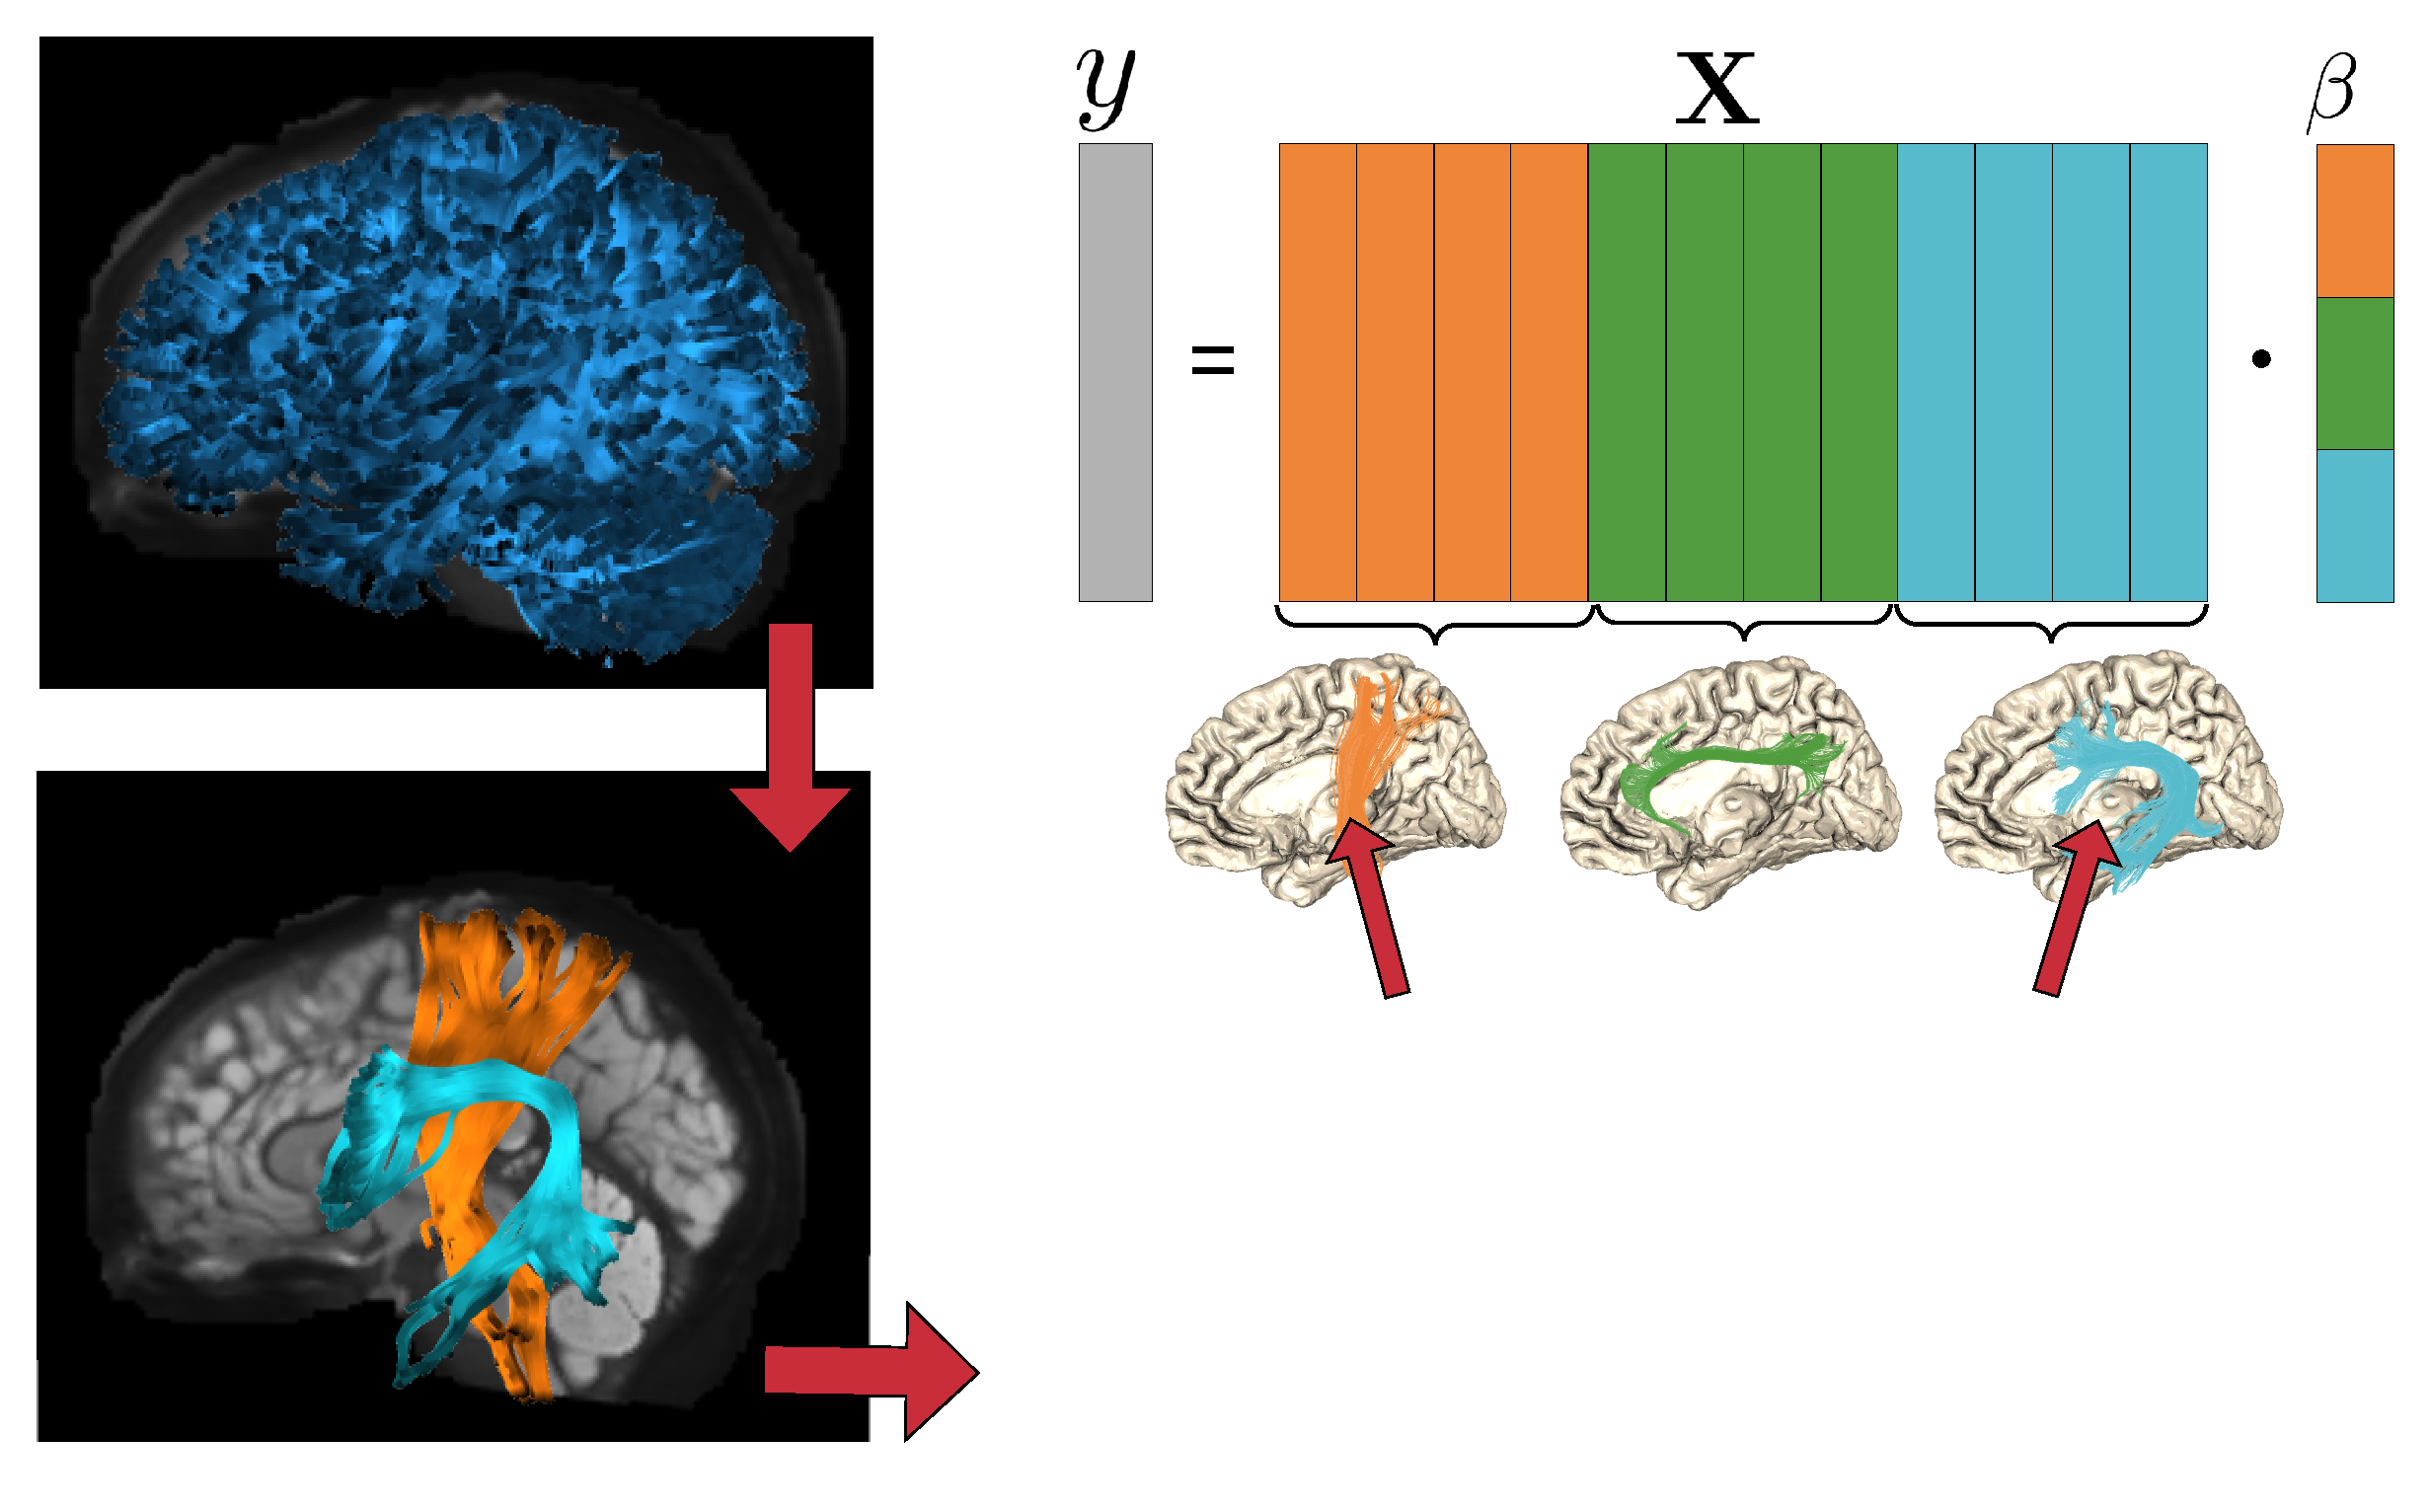
\includegraphics[width=0.98\columnwidth]{methods-brains.pdf}
    }
    \vspace{-9.75cm}
    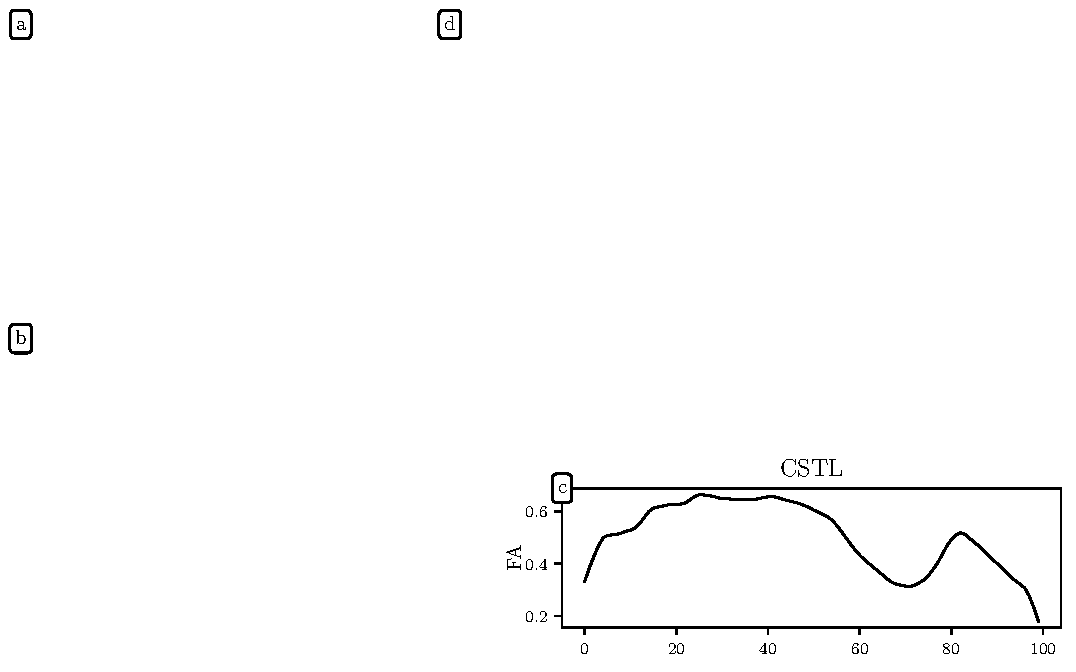
\includegraphics[width=\columnwidth]{method-quad.pdf}
    {\phantomsubcaption\label{fig:methods:tractogram}}
    {\phantomsubcaption\label{fig:methods:cst}}
    {\phantomsubcaption\label{fig:methods:tract-profile}}
    {\phantomsubcaption\label{fig:methods:group-structure}}
    \caption{{\bf Tractometry data flow}
        \label{fig:methods}
        {\bf (a)} Whole brain tractography generates streamlines approximating
        the trajectories of white matter connections.
        {\bf (b)} Tractometry classifies these streamlines into anatomical bundles.
        In this case, we show the left corticospinal tract (CSTL) over a mid-saggital
        anatomical slice.
        {\bf (c)} Tractometry further extracts bundle profiles,
        quantifications of various diffusion metrics along the length of the
        fiber bundle. Here, we show one subject's fractional anisotropy (FA)
        profile for CSTL.
        {\bf (d)} the phenotypical target data and tractometric features can
        be organized into a linear model, $\hat{y} = \mathbf{X}
        \hat{\beta}$. The feature matrix $\mathbf{X}$ is color-coded
        to reveal a natural group structure: the left (orange) group
        contains $k$ features from the CSTL, the middle (green) group
        contains $k$ features from the left cingulum cingulate (CGCL),
        and the right (blue) group
        contains $k$ features from the left arcuate (ARCL). The coefficients in
        $\hat{\beta}$ follow the same natural grouping.
        % Cross-validation:
        % we evaluate model quality using a nested $k$-fold cross validation
        % scheme. At level-0, the input data is decomposed into $k$
        % shuffled groups and optimal hyperparameters are found for the level-0
        % training set.
        % To avoid overfitting, the optimal hyperparameters are themselves
        % evaluated using a cross-validation scheme taking place
        % at level-1 of the decomposition, where each
        % level-0 training set is further decomposed into five shuffled
        % groups. For the ALS and WH data, $k=10$, while for the HBN and
        % Cam-CAN data, $k=5$.
    }
\end{figure}

Non-invasive methods for measuring human brain structure and function have
revolutionized our understanding of brain function. These measurements
have demonstrated that interactions between networks of brain regions give rise
to coordinated information processing and to the complex adaptive behavior that
characterizes human cognition. Diffusion-weighted Magnetic Resonance Imaging
(dMRI) provides a unique view into the physical properties of the connections
that comprise these networks, by sensitizing the measurement to the directional
diffusion of water in each voxel \cite{wandell2016clarifying}.
% While the measurements are usually conducted
% with voxels at the millimeter scale, water molecules within each voxel
% diffuse with characteristic lengths at the micrometer scale, providing
% aggregate information about the physical structure of the white matter,
% including the density of axons and distribution of fiber
% orientations within each voxel \cite{wandell2016clarifying}. Even though
% metrics derived from diffusion measurements are ambiguous in terms
% of their underlying biological interpretation \cite{Jones2013-xv},
% analyzing the variance in these properties has proven useful in
% characterizing individual differences in cognitive function,
% characterizing differences between populations and detecting brain
% abnormalities associated with disease \cite{Thomason2011-qn}.
Methods for computational tract-tracing from diffusion MRI, or tractography,
combine the estimates of fiber orientations in each voxel to form streamlines
that traverse the volume of the white matter~\cite{Conturo1999-je,
Mori2002-qi}. A variety of methods can be used to delineate the
trajectory of major neural pathways among these
streamlines~\cite{yeatman2012tract}.
% These methods have been under increased scrutiny and
% several lines of investigation have raised critiques of their validity
% \cite{Maier-Hein2017-vb, Thomas2014-ki}. On the other hand, there
% have been efforts to shore up the inferences made with these methods
% \cite{Pestilli2014NatMeth, Takemura2016-sh, Smith2013-nc, Smith2015-cx,
% Smith2015-zt, Rheault2018-wk}. Importantly, though discovering novel
% tracts requires extraordinary evidence, and delineating
% the exact cortical termination of the streamlines in the gray matter
% is still prone to error, there is little dispute that tractography
% can accurately define the location of several major white matter
% tracts that are known to exist within the core of the white matter
% \cite{Maier-Hein2017-vb, Catani2002-vu}.
\emph{Tractometry} uses the results of tractography and models
of tissue biophysics based on the patterns of diffusion in each measurement
voxel to assess the physical properties of the white matter along specific
pathways~\cite{Bells2011-cf}.
%Though there are several different available implementations of this overall
%idea, the principles are similar \cite{yeatman2012tract, Yendiki2011-ay,
%Wassermann2016-iv, ODonnell2009-uu}: tractometry begins by delineating
% the parts of the white matter that belong to different major ``tracts''
% (i.e. anatomical or functional groups of white matter fibers), such as
% the corticospinal tract or arcuate fasciculus, assigning tractography
% generated streamlines to ``bundles,'' which approximate the anatomical
% tracts, and sampling biophysical properties, such as fractional
% anisotropy (FA) or mean diffusivity (MD), along the length of these bundles.
% The parts of the white matter that belong to different major tracts
% (i.e. anatomical or functional groups of white matter fibers), such as
% the corticospinal tract or arcuate fasciculus, assigning tractography
% generated streamlines to ``bundles,'' which approximate the anatomical
% tracts, and sampling biophysical properties (such as fractional
% anisotropy or mean diffusivity) along the length of these bundles.
In some previous tractometry-based studies, tissue properties along the
length of each tract were summarized by taking the mean along each
bundle, but there is a large body of evidence showing that there is
systematic variability in the values of diffusion metrics along the
trajectory of each bundle. This justifies retaining the individual
samples along the length of each bundle \cite{yeatman2012tract,
colby2012, ODonnell2009-uu}. While this retains important information
about each individual's white matter, it also presents statistical
challenges due to the dimensionality of the data. In past work,
comparisons between groups or across individuals were done
independently at each node of each bundle, for each
diffusion metric. This approach is exhaustive, but
statistical power is compromised by a multiple comparison problem
\cite{colby2012, Nichols2002-zu, Nichols2003-yy}. An alternative that
circumvents the multiple comparison problem is to select just a few
tracts to compare in each individual, or even
segments of these tracts based on \emph{a priori} hypotheses. This
approach is appropriate when the biological basis of the process
of interest is relatively well understood (for a recent example, see
\cite{huber2018rapid}). Sometimes, these approaches are combined: a
bundle is selected based on \emph{a priori} knowledge, and all the data
in the bundle of interest are used together to fit a model that can
predict differences between individuals \cite{dayan2016profilometry}.

% Different approaches can be taken to resolving this challenge. For
% example, Colby and colleagues \cite{colby2012} used a non-parametric
% approach to
% correct for family-wise error across the different possible comparisons
% \cite{Nichols2002-zu, Nichols2003-yy}.
% Based on tractometry, researchers may choose to compare different individuals
% to each other. This is usually done according to one of the following
% approaches:
% \begin{enumerate}
% \item Mass univariate approaches: In this approach


% \item Region of interest(ROI)-based approaches:
% An alternative that
% circumvents the multiple comparison problem is to select just a few
% tracts to compare in each individual, or even focusing on particular
% segments of these tracts based on \emph{a priori} hypotheses. This
% approach is very powerful when the biological basis of the process
% of interest is relatively well understood (for a recent example, see
% \cite{huber2018rapid}).

% \item ROI-based selection, followed by multivariate analysis: Here,
% an ROI is selected based on \emph{a priori} knowledge, and all the
% nodes or voxels in the ROI are used together to fit a model that can
% predict differences between individuals. An example of that is the
% ``profilometry'' framework, in which different diffusion metrics
% from a single tract are combined together to provide input to a
% multivariate analysis of covariance, and linear discriminant analysis
% \cite{dayan2016profilometry}.

%\end{enumerate}

The present work aims to balance predictive accuracy with descriptive power
\cite{Murdoch2019-ax, Breiman2001-uz} by capitalizing on all of the available
data across all bundles, while also retaining and elucidating spatial
information about the locations that are most informative for discriminative
performance. To do so, we use a linear modeling approach, which aims to
redict phenotypical variance in a group of subjects (or classify group
membership), based on a linear combination of the features estimated with
tractometry.

% Generally speaking, analysis methods should balance predictive
% accuracy with descriptive power \cite{Murdoch2019-ax, Breiman2001-uz}.
% Accordingly, tractometry analysis should simultaneously capitalize on
% all the data across all tracts to make the best possible prediction,
% while also retaining and elucidating spatial information about the
% locations that are most informative for a prediction. In the present
% work, we developed a novel framework for analysis of tractometry that
% simultaneously selects the features for analysis, and fits a model
% to these features. We use a linear modeling approach, which aims to
% predict phenotypical variance in a group of subjects, based on a linear
% combination of the features estimated with tractometry.

Using this approach, we first need to deal with the large and
asymmetric dimensionality of the data: tractometry data usually has
many more features (i.e., number of measurements per individual) than
samples (number of subjects), which makes inferences from the data
about phenotypical differences between individuals ill-posed. This
regime is the target of several statistical learning techniques, and
is often solved by various forms of regularization.

% For example, Tikhonov regularization shrinks the solution such that the sum of
% squared contributions from the individual features are minimized
% \cite{Hoerl2000-ij}. Another solution to the problem is provided by
% the

The Lasso algorithm minimizes the sum of the absolute values of
contributions of each feature \cite{Tibshirani1996-qs}. This
tends to shrink to zero the contributions of many of the features,
providing results that are both accurate and interpretable. When
additional structure is available in the organization of the data,
regularization algorithms can take advantage of this structure. For
example, if the features lend themselves to a natural division into
different groups, the Group Lasso (GL) can be used to select groups
of features, rather than individual features \cite{Yuan2006-ky}.
The Sparse Group Lasso (SGL) elaborates on this idea by providing
control both of group sparsity, as well as overall sparsity of the
solutions \cite{simon2013sgl}. Because the features measured with
tractomery lend themselves to grouping based on the tracts from which
each measurement is taken, GL and SGL provide useful tools
for linear model fitting in problems of this form. Here we, first,
develop an implementation of SGL that is well suited to the analysis of
tractometry data and, second, demonstrate the power and flexibility of
this approach by applying it to both classification
and continuous prediction problems.

\subsection*{Results}

\begin{figure*}
    \vspace{3cm}
    \rlap{
        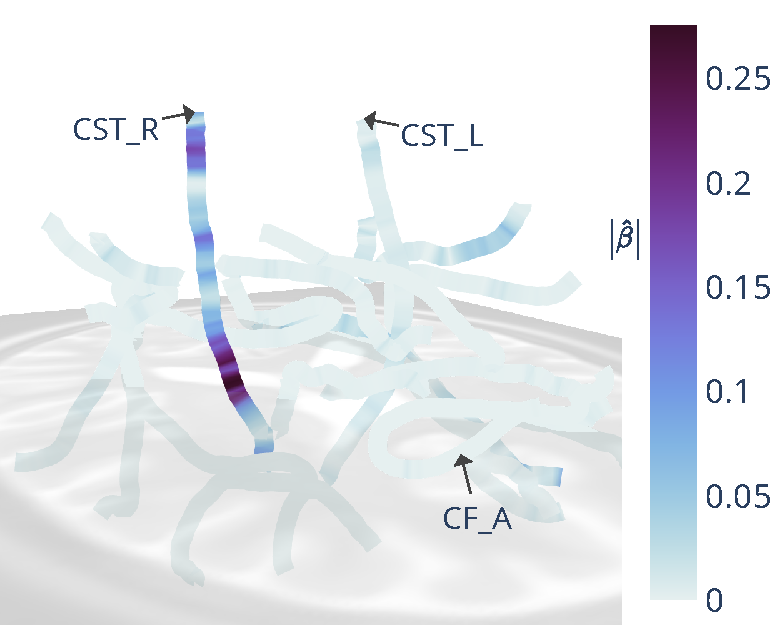
\includegraphics[width=0.33\textwidth]{als_coefs.pdf}
    }
    \vspace{-8.4cm}
    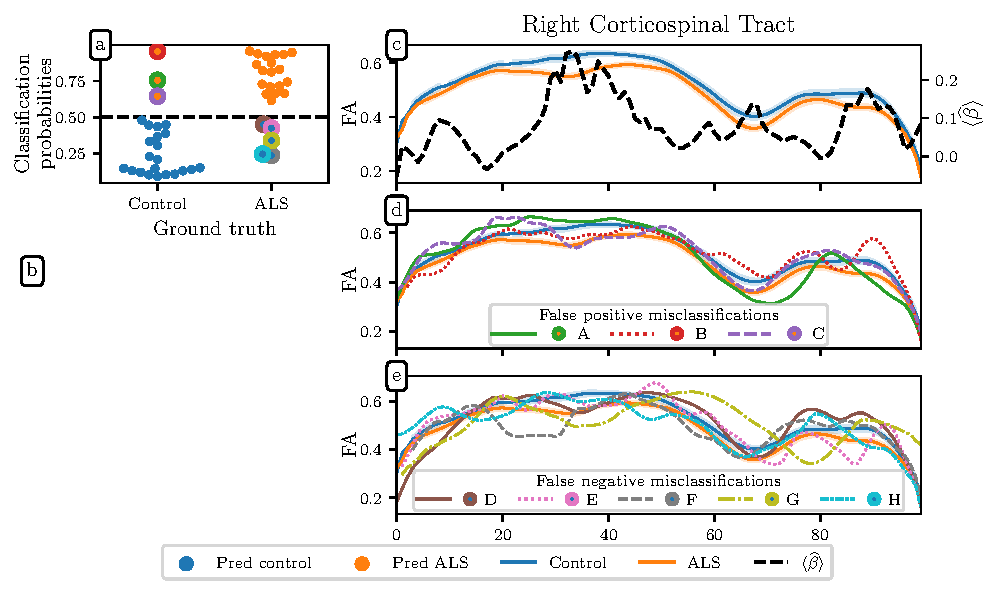
\includegraphics[width=\textwidth]{als_results.pdf}
    {\phantomsubcaption\label{fig:class-results:probs}}
    {\phantomsubcaption\label{fig:class-results:coefs3d}}
    {\phantomsubcaption\label{fig:class-results:tract-profiles}}
    {\phantomsubcaption\label{fig:class-results:false-positives}}
    {\phantomsubcaption\label{fig:class-results:false-negatives}}
    \caption{%
        {\bf SGL accurately and interpretably predicts ALS diagnosis.}
        \label{fig:class-results}
        {\bf (a)} Classification probabilities for ALS diagnosis, with
        controls on the left, patients on the right, predicted controls in
        blue, and predicted patients in orange. That is, orange dots on the left
        represent false positives, while blue dots on the right represent
        false negatives. We achieve {\protect\alsAccuracy}\% accuracy with an
        ROC AUC of {\protect\alsRocAuc}.
        {\bf (b)} SGL coefficients are presented on the core fibers of major
        fiber bundles. They exhibit high group sparsity and are concentrated
        in the FA of the CST. The brain is oriented with the right hemisphere
        in the foreground and anterior to the right of the page. The CSTL,
        CSTR, and CFA bundles are indicated for orientation.
        {\bf (c)} SGL identifies three portions of the CST as important,
        where $\hat{\beta}$ (dashed line, right axis) has large values. These
        are centered around nodes 30, 65, and 90, corresponding to locations
        of substantial differences in FA between the ALS and control groups
        (shaded areas indicates standard error of the mean).
        {\bf (d)} Bundle profiles for false positive classifications. Line
        colors correspond to the marker edge color in the top left plot.
        These individuals have reduced FA in the CST portions which SGL
        identified as important. Their misclassification is coherent with the
        feature importance and the group differences in FA.
        {\bf (e)} Individual bundle profiles for false negative
        classifications. These individuals have bundle profiles which
        oscillate between the group means.
    }
\end{figure*}

We developed a method for analyzing dMRI tractometry data that uses the Sparse
Group Lasso (SGL) to select features that are sparse both at the group (bundle) level, as well as overall.
We demonstrate the use of this method on four different datasets in
both a classification setting and a regression setting.

\subsubsection*{SGL accurately detects ALS from tractometry data}

Using data from a previous study of patients with amyotrophic lateral sclerosis (ALS)~\cite{sarica2017corticospinal}, we tested the performance of SGL in a
classification setting. The previous study predicted ALS status with a mean
accuracy of 80\% using a random forest algorithm based on \emph{a priori}
selection of features only within the CST bundle-of-interest.
SGL delivers improved predictive performance, with a cross-validated accuracy of {\alsAccuracy}\% and an area under the receiver operating characteristic curve (ROC AUC) of {\alsRocAuc}, without the need for \emph{a priori} feature engineering (Figure \cref{fig:class-results:probs}). In addition to this
classification performance, SGL also identifies the white matter tracts most
important for ALS classification. The relative importance of white matter
features is captured in the $\beta$ coefficients from \cref{supp:eq:sgl} of
the supplemental material \cite{supplement}.
\Cref{fig:class-results:tract-profiles} depicts these coefficients along the
right CST, plotted over the FA values for the control and ALS subject groups.
We find that SGL selects FA metrics in the corticospinal tract and
particularly in the right corticospinal tract as most important to ALS
classification, confirming previous findings \cite{van2011upper,
toosy2003diffusion, sarica2014tractography, sage2007quantitative,
sage2009quantitative, karlsborg2004corticospinal, ellis1999diffusion,
cosottini2005diffusion, ciccarelli2009investigation, abe2010voxel} and
identifying the portions of the brain that were selected \emph{a priori} in
the previous study from which we obtained the data
\cite{sarica2017corticospinal}.
\todo{Adam: Add sentence comparing to pure lasso results. Lasso accuracy: 0.76; lasso ROC AUC: 0.76}

The $\beta$ coefficients exhibit high bundle level sparsity; only some
bundles are important, which can be be confirmed by observing the value of
$\alpha$, the regularization hyperparameter that controls the mixture of the
Group Lasso and lasso penalties, selected through nested cross-validation
(see \cref{supp:eq:sgl} of the supplemental material \cite{supplement}).
If $\alpha$ is closer to zero, it indicates that the phenotype in question
preferentially correlates with only a few groups of covariates. For the ALS
dataset, $\alpha = $ \alsLRatio, confirming that the white matter correlates
of ALS reside mostly in one bundle, namely the CST.

Analyzing the ways in which the model mislabels individuals also provides
insight. We found that mislabelled subjects are outliers relative to their
group with respect to diffusion features of the CST (Figure
\Cref{fig:class-results:false-positives,fig:class-results:false-negatives}).
The false positive classifications have reduced FA in one or more of the three
sections of the CST where $\norm*{\hat{\beta}}$ is large
\cref{fig:class-results:tract-profiles}. The false negative subjects have FA
profiles that oscillate between the two group means. Thus, when the SGL
method predicts incorrectly this is done in a comprehensible manner.

\begin{figure*}
    \vspace{3.65cm}
    \rlap{
        \hspace{1cm}
        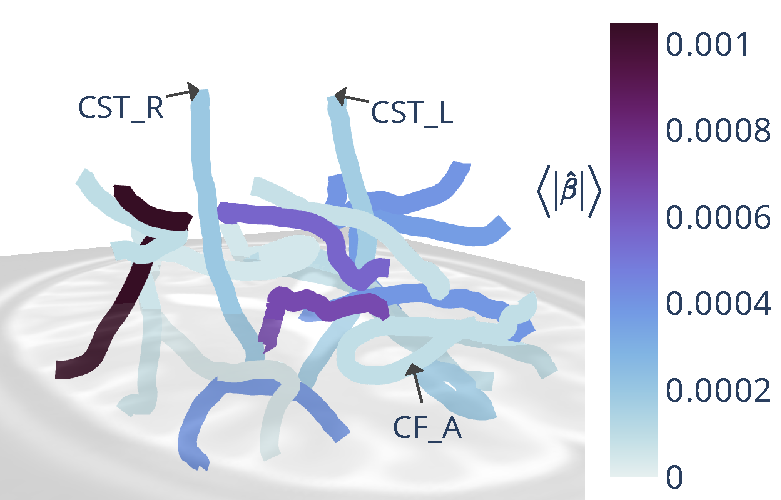
\includegraphics[width=0.275\textwidth]{wh_coefs.pdf}
        \hspace{0.25em}
        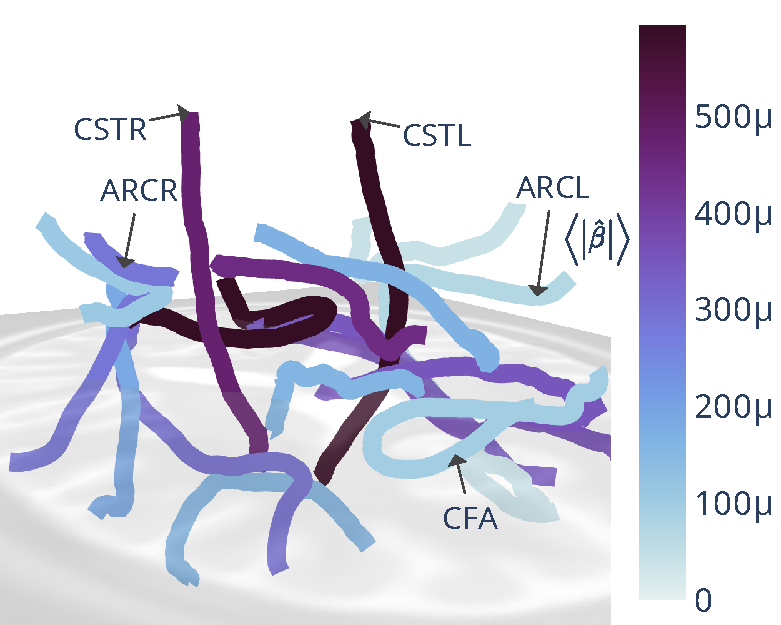
\includegraphics[width=0.275\textwidth]{hbn_coefs.pdf}
        \hspace{0.25em}
        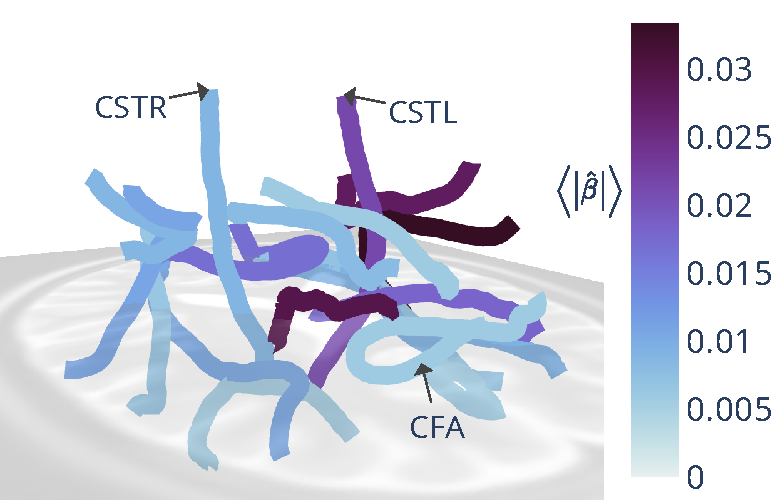
\includegraphics[width=0.275\textwidth]{camcan_coefs.pdf}
    }
    \vspace{-7.3cm}
    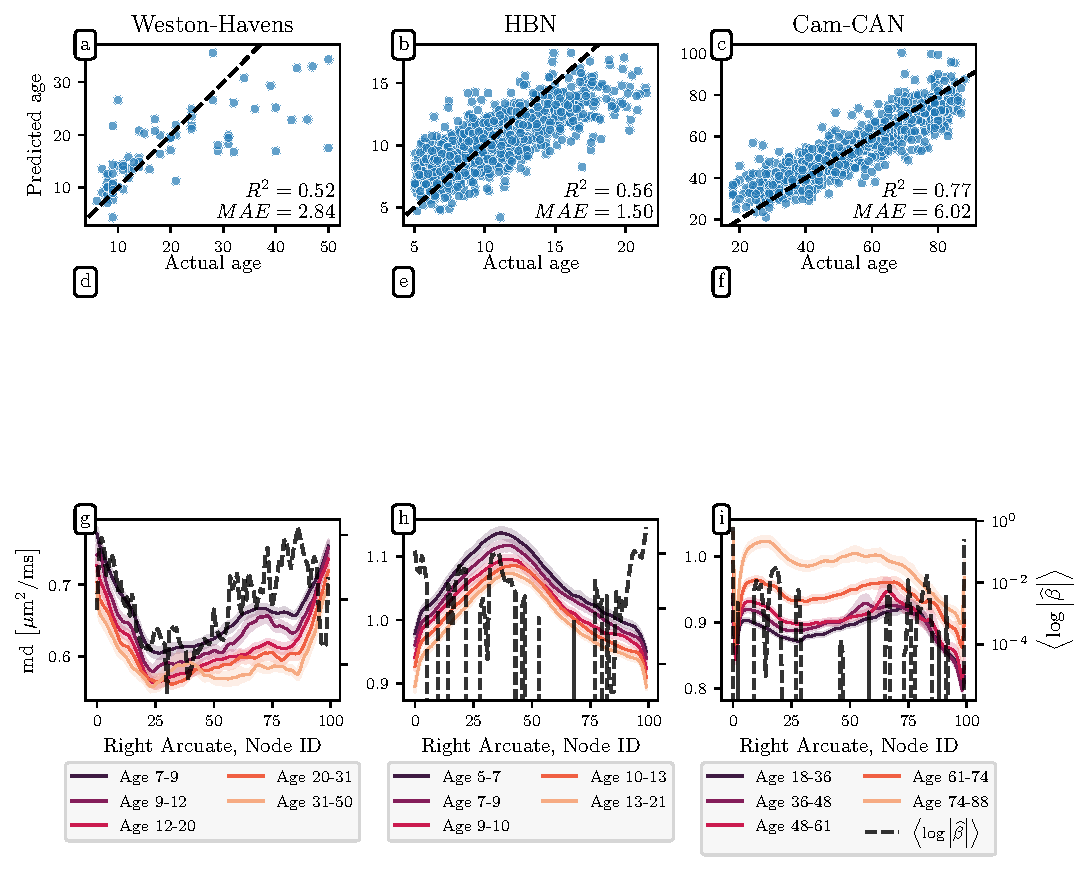
\includegraphics[width=\textwidth]{regression_scatter.pdf}
    {\phantomsubcaption\label{fig:age-results:wh-scatter}}
    {\phantomsubcaption\label{fig:age-results:hbn-scatter}}
    {\phantomsubcaption\label{fig:age-results:cc-scatter}}
    {\phantomsubcaption\label{fig:age-results:wh-coefs3d}}
    {\phantomsubcaption\label{fig:age-results:hbn-coefs3d}}
    {\phantomsubcaption\label{fig:age-results:cc-coefs3d}}
    {\phantomsubcaption\label{fig:age-results:wh-profile}}
    {\phantomsubcaption\label{fig:age-results:hbn-profile}}
    {\phantomsubcaption\label{fig:age-results:cc-profile}}
    \caption{%
        {\bf Predicting age with tractometry and SGL.}
        \label{fig:age-results}
        {\bf (top)} The predicted age vs. true age of each individual from the test
        splits (i.e., when each subject's data was held out in fitting the
        model) for the {\bf (a)} WH, {\bf (b)} HBN, and {\bf (c)} Cam-CAN
        datasets; an accurate prediction falls close to the $y=x$ line
        (dashed). The mean absolute error (MAE) and coefficient of
        determination $R^2$ are presented in the lower right of each scatter
        plot.
        {\bf (middle)} Feature importance for predicting age from tractometry in
        the {\bf (d)} WH, {\bf (e)} HBN, and {\bf (f)} Cam-CAN datasets.
        The orientation of the
        brain is that same as in \cref{fig:class-results:coefs3d}, however because
        the coefficients exhibit high global sparsity (as opposed to group
        sparsity), we plot the mean of the absolute value of $\hat{\beta}$
        for each bundle on the core fiber. The global distrubution of the
        $\hat{\beta}$ coefficients reflects the fact that aging is not
        confined to a single white matter bundle.
        {\bf (bottom)} Age quintile bundle profiles for the {\bf (g)} WH,
        {\bf (h)} HBN, and {\bf (i)} Cam-CAN datasets.
    }
\end{figure*}

\subsubsection*{SGL accurately predicts age from tractometry data}

To test the performance of SGL with tractometry data in a continuous
regression task, we focus here on the prediction of biological age in three
datasets named WH, HBN, and Cam-CAN (see supplemental material
\cite{supplement} for a description of each dataset). Prediction of ``brain
age'' is a commonly undertaken task in neuroimaging machine learning, in part
because these predictions, and deviations therefrom, may be diagnostic of
overall brain health (for a review, see Cole et al.~\cite{Cole2019-rz}).
However, as Nelson et al.~\cite{nelson2019biomarkers} have observed, aging
biomarkers are subject to unique challenges and tend to be noncausative. Our
interest in aging here relies on its utility as a methodological benchmark.
Biological age operates on a natural scale, with meaningful and easily
understood units, and it's popularity as a machine learning target makes it
valuable for comparisons with other studies.

The WH \cite{yeatman2014lifespan}, HBN \cite{alexander2017open}, and Cam-CAN
\cite{shafto2014cambridge,taylor2017cambridge} datasets used here contain
data from 76, 978, and 640 subjects, respectively, ranging from 6-50, 5-21,
and 18-88 years of age, respectively. In each case, biological age was used
as the predicted variable $y$. SGL was fit to the tractometry-extracted
features FA and MD in 18 major brain tracts, with diffusion metrics extracted
from diffusion tensor imaging (DTI) for the WH dataset and diffusion kurtosis
imaging (DKI) \cite{jensen2005diffusion} for the HBN and Cam-CAN datasets.

To evaluate the fit of the model, we used a nested cross-validation
procedure. In this procedure, batches of subjects are held out. For each
batch (or fold), the model is fully fit without this data. Then, once the
parameters are fixed, the model is applied to predict the ages of held out
subjects based on the linear coeffiecients. This scheme automatically finds
the right level of sparsity and fits the coefficients to the ill-posed linear
model, while guarding against overfitting. SGL accurately predicts the age of
the subjects in this procedure, with a median absolute error of {\whMae},
{\hbnMae}, and {\camcanMae} years for the WH, HBN, and Cam-CAN datasets,
respectively and coefficients of determination $R^2 = $ {\whRsq} , {\hbnRsq},
and {\camcanRsq}, respectively (see \cref{fig:age-results}, top panels). The
predictions for Cam-CAN are competitive with a recent state of the art
prediction \cite{mcpherson2020single}, which used streamline density to
estimate the brain's structural connectivity and achieved $R^2 = 0.63$. The
median absolute errors are also lower than the results of a recent study that
predicted age in a large sample that included the Cam-CAN data, and was based
on diffusion MRI features \cite{Richard2018-ux}.
\todo{Adam: Add sentence comparing to pure lasso results.
Lasso WH R2: 0.47; Lasso WH MAE: 4.43;
Lasso HBN R2: 0.57; Lasso HBN MAE: 1.49;
Lasso CC R2: 0.70; Lasso CC MAE: 6.08;
}

In contrast to the ALS classification case, the selected $\alpha$ values
indicate high global sparsity over group sparsity, with $\alpha = $
{\whLRatio}, {\hbnLRatio}, and {\ccLRatio}, for the WH, HBN, and Cam-CAN
datasets, respectively. The model weights are distributed over many different
tracts and dMRI tissue properties (see
\cref{fig:age-results:wh-coefs3d,fig:age-results:hbn-coefs3d,fig:age-results:cc-coefs3d}
and supplemental material
\cref{supp:fig:wh-bp:md,supp:fig:wh-bp:fa,supp:fig:hbn-bp:md,supp:fig:hbn-bp:fa,supp:fig:cc-bp:md,supp:fig:cc-bp:fa}).
This demonstrates that SGL is not coerced to produce overly sparse results
when a more accurate model requires a dense selection of features.
Furthermore, inspecting the portions of bundles with larger coefficients in
\cref{fig:age-results:wh-profile,fig:age-results:hbn-profile,fig:age-results:cc-profile}
reveals that SGL selects informative regions where diffusion properties are
different between the age quintiles.

\subsection*{Discussion}

We present here a novel method for analysis of dMRI tractometry data that
relies on the Sparse Group Lasso \cite{simon2013sparse} to make accurate
predictions of phenotypic properties of individual subjects while,
simultaneously, identifying the features of the white matter that are
most important for this prediction. The method is data-driven and it is broadly applicable to a wide range of research questions: it
performs well in predicting both continuous variables, such as biological
age, as well as categorical variables, such as whether a person is a patient
or a healthy control. In both of these cases, SGL out-performs previous
algorithms that have been developed for these tasks
\cite{sarica2017corticospinal, Richard2018-ux, mcpherson2020single}. The
nested cross-validation approach used to fit the model and make both
predictions and inferences from the model guards against overfitting and
tunes the degree of sparseness required by the algorithm. This means that SGL
can accurately describe phenomena that are locally confined to a particular
anatomical location or diffusion property (e.g., FA in the CST) as well as
phenomena that are widely distributed amongst brain regions and measured
diffusion properties.

Specifically, we demonstrated that the algorithm correctly detects the fact
that ALS, which is a disease of lower motor neurons, is localized to the
cortico-spinal tract. This recapitulates the results of previous analysis of
these same data, using a bundle-of-interest approach
\cite{sarica2017corticospinal}. In contrast, for the analysis of biological
age, the coefficients identified by the algorithm are very widely distributed
across many parts of the white matter, mirroring previous results that show a
large and continuous distribution of life-span changes in white matter
properties \cite{yeatman2014lifespan}.

One drawback of our approach is also evident in the age regression results.
There are portions of the bundle profiles in
\cref{fig:age-results:wh-profile,fig:age-results:hbn-profile,fig:age-results:cc-profile}
for which the $\hat{\beta}$ coefficients are zero but for which the bundle
profiles clearly contain an age differentiating signal. While SGL correctly
identifies certain features as important, it is not guaranteed to identify
\emph{all} of the important features. It will identify a parsimonious set of
important features, dense enough to predict the phenotype and sparse enough
(at either the group or global level) to satisfy the sparsity constraints.

Taken together, these results demonstrate the promise of the
group-regularized regression approach. Even at the scale of dozens of
subjects, the results provided by SGL are both accurate, as well as
interpretable \cite{Murdoch2019-ax}: tractometry capitalizes on domain
knowledge to engineer meaningful features; SGL scores these features based on
their relative importance; enables a visualization of these feature
importance scores in the anatomical coordinate frame of the bundles (e.g.,
\cref{fig:class-results:coefs3d,fig:age-results:wh-coefs3d,fig:age-results:hbn-coefs3d,fig:age-results:cc-coefs3d})
and provides a means to understand model errors (e.g.,
\cref{fig:class-results:false-positives,fig:class-results:false-negatives}) .
Thus, this multivariate analysis approach achieves high
cross-validated accuracy for precision medicine applications of dMRI data and identifies relevant features of brain anatomy that can further our
neuroscientific understanding of clinical disorders.

Neuroscience has entered an era in which consortium efforts are amassing
large datasets of high-quality dMRI measurements to address a variety of
scientific questions \cite{jernigan2016ping, jernigan2018abcd,
alexander2017open, Miller2016-hw, VanEssen2012}, but the volume and
complexity of these data pose substantial challenges. Tractometry
followed by analysis with SGL provide a promising approach to
distill meaningful insights from the wealth of data measured in these efforts.

SGL has many other potential applications in neuroscience, because
of the hierarchical and grouped nature of many data types that are
collected in multiple sample points within anatomically-defined areas.
For example, this method may be useful to understand the relationship
between fMRI recordings and behavior, where activity in each voxel
may co-vary with voxels within the same anatomical region and form
features and groups of features. Similarly, large-scale multi-electrode
recordings of neural activity in awake behaving animals are becoming
increasingly feasible \cite{steinmetz2018distributed, Jun2017-gv} and
these recordings can form features (neurons) and groups (neurons within
an anatomical region).

% More ambitiously perhaps, this approach may be
% used to understand the role of correlations in so-called resting-state
% fMRI time-series and behavior, where pairwise correlations between
% voxels in different anatomical regions are features in the matrix and
% features may be grouped by pairs of anatomical regions. Given the large
% number of voxels in the surface of the gray matter and given that
% correlations increase the number of features by a factor of $n^2$, this
% would pose a challenging problem to solve using SGL.

The results we present here also motivate extensions of the method using more
sophisticated cost functions. For example, the fused sparse group lasso (FSGL)
\cite{zhou2012} extends SGL to enforce additional spatial structure: smoothness
in the variation of diffusion metrics along the bundles. As brain measurements
include additional structure (for example, bilateral symmetry), future work
could also incorporate overlapping group membership for each entry in the tract
profiles \cite{Rao2014-xm}. For example, a measurement could come from the
corpus callosum, but also from the right hemipshere. This would also require
extending the cost function used here to incorporate these constraints.
Similarly, unsupervised dimensionality reduction of tractometry data (e.g.,
\cite{Chamberland2019-mu}) could also benefit from constraints based on
grouping.

The method is packaged as open-source software called AFQ-Insight that is
openly available \todo{Ariel: add URL}, and provides a clear API to allow for
extensions of the method. The sofware integrates within a broader automated
fiber quantification software ecosystem: AFQ \cite{yeatman2012tract} and
pyAFQ (https://yeatmanlab.github.io), which extract tractometry data from raw
and processed dMRI datasets, as well as AFQ-Browser, which visualizes
tractometry data and facilitates sharing of the results of dMRI studies
\cite{yeatman2018browser}. To facilitate reproducibility and ease use of the
software, the results presented in this paper are also provided in
\url{https://github.com/richford/AFQ-Insight/tree/master/examples/preprint-notebooks}
\todo{Adam: Update notebooks}
as a series of Jupyter notebooks \cite{kluyver2016jupyter}.

\subsection*{Methods}

Methods and associated references are available in the supplemental material.

\subsection*{Acknowledgments}

This work was supported by BRAIN Iniative grant 1RF1MH121868-01 from the
National Institutes for Mental Health, by a grant from the Gordon \& Betty
Moore Foundation and the Alfred P. Sloan Foundation to the University of
Washington eScience Institute Data Science Environment, and by the Google
Cloud Platform Academic Research Credits Program. We would like to thank
Scott Murray for a useful discussion of the SGL method and Mareike Grotheer
for helpful comments on the manuscript.

\subsection*{Author contribution statement}

All authors contributed extensively to the work presented in this paper.

\printfigures

\bibliographystyle{naturemag}
\bibliography{paper}

\end{document}
